\documentclass{article}

% for multilangual document, change desired language here
\newcommand{\inGerman}[1]{#1}
\newcommand{\inEnglish}[1]{}


\usepackage[utf8]{inputenc}
\inGerman{\usepackage[ngerman]{babel}}
\usepackage[urlcolor=blue,linkcolor=green]{hyperref}
\usepackage{geometry} \geometry{a4paper, top=25mm, left=25mm, right=25mm, bottom=25mm}
\usepackage{tikz} % for drawing graph
\usepackage{fancyhdr}
\usepackage{listings}
\usepackage{todonotes}
\usepackage{hyperref}

% new page after each section
\usepackage{titlesec}
\newcommand{\sectionbreak}{\clearpage}

\lstset{
  breaklines=true,
% basicstyle=\footnotesize,         % the size of the fonts that are used for the code
  numbers=left,                     % where to put the line-numbers
  numberstyle=\tiny\color{red}      % the style that is used for the line-numbers
}

% set margins

\begin{document}
\begin{titlepage}
	\begin{center}
		\vspace*{30mm}
\inEnglish{
		\textbf{\Huge{(inofficial) \\}}
		\textbf{\Huge{\href{http://retroshare.sourceforge.net/}{RetroShare} User Manual}} \\[5mm]
		\large{last update: \today} \\[85mm]
		\vfill
		\small{written by \href{http://yet-another-nerd-blog.de}{Klaus Eisentraut}, Budlack and \href{https://sourceforge.net/users/marcusls}{MarcusLS}} \\
		\small{starting in April 2012} \\
		\small{Licence: \href{http://creativecommons.org/licenses/by-sa/3.0/de/}{cc by-sa}}
}
\inGerman{
		\textbf{\Huge{(inoffizielles) \\}}
		\textbf{\Huge{Benutzerhandbuch \href{http://retroshare.sourceforge.net/}{RetroShare}}} \\[5mm]
		\large{Version vom \today} \\[85mm]
		\vfill
		\small{geschrieben von \href{http://yet-another-nerd-blog.de}{Klaus Eisentraut}, Budlack und \href{https://sourceforge.net/users/marcusls}{MarcusLS}} \\
		\small{im April 2012} \\
		\small{Lizenz: \href{http://creativecommons.org/licenses/by-sa/3.0/de/}{cc by-sa}}
}
	\end{center}
\end{titlepage}

\clearpage
\tableofcontents
\clearpage
% change parindent and parskip
\setlength{\parindent}{0cm} \setlength{\parskip}{6pt}
%
% now the actual content
%
\inGerman{\section{Über dieses Dokument}}
\inEnglish{\section{About this document}}
\inGerman{Dieses Dokument ist eine inoffizielle Anleitung für das Computer-Programm \href{http://retroshare.sourceforge.net/}{RetroShare}.}
\inEnglish{This document is an inofficial user manual for the program \href{http://retroshare.sourceforge.net/}{RetroShare}.}

\inGerman{Wir haben dieses Handbuch in \LaTeX geschrieben, weil wir RetroShare für ein geniales Projekt mit großem Potenzial halten und es unterstützen möchten.
Da die Entwickler keine Spenden annehmen, möchte wir hiermit unseren Beitrag zu Retroshare leisten.
Sämtliches Wissen über RetroShare haben wir uns durch Ausprobieren, Lesen von RetroShare-internen Foren und gelegentliches in den Quellcode schauen angeeignet.
Wir sind insbesondere keine Entwickler von RetroShare und es ist möglich, dass hier einige Details nicht ganz richtig sind, oder sich im Zuge der Entwicklung mitlerweile geändert haben.}
\inEnglish{We wrote this manual in \LaTeX, because we are big fans of RetroShare and we think it has great potential.
As we can't support the development by donating some money to the developers and/or coding, this is our way to support it.
We got our knowledge about RetroShare mainly via try and error, reading the forums and looking in the code sometimes.
We are NOT developers of RetroShare and some minor details here might be wrong or have changed over time.}

\inGerman{Wenn du also in diesem Dokument inhaltliche Fehler gefunden hast, wäre wir um eine kurze Rückmeldung sehr dankbar.
Auch wenn du mithelfen möchtest, dieses Dokument zu verbessern (z.B. vervollständigen, Übersetzung in andere Sprachen, schöneres Deutsch xD ...) und zumindest die Grundlagen von \LaTeX kannst, so nehme bitte mit uns Kontakt auf. Kontaktdaten befinden sich auf Klaus privaten Blog unter der Adresse \url{http://yet-another-nerd-blog.de/legal-notice/}.}
\inEnglish{If you notice an error in this document, we'd appreciate a short feedback.
If you want to help improving this document and you know at least the basics of \LaTeX, so contact us. Klaus's contact information can be found on his private blog at \url{http://yet-another-nerd-blog.de/legal-notice/}.
A native english speaker would be appreciated for proof-reading :)}

\newpage
\section{\inGerman{Eine kurze Einführung in OpenPGP}\inEnglish{A short introduction to OpenPGP}}

\inGerman{Da RetroShare stark auf OpenPGP und dessen Funktionsweise aufbaut, soll hier eine (sehr kurze) Einführung dazu stattfinden.
Wer sich damit schon auskennt, kann ohne weiteres zum nächsten Kapitel springen.
Über GnuPG und Email-Verschlüsselung findet man im Internet schon Dokumente zuhauf, wir wollen hier nur auf die absoluten Grundlagen eingehen.}
\inEnglish{Since RetroShare makes heavy use of OpenPGP, we want to make a (very) short introduction to asymmetric encryption here.
If you know about OpenPGP already, you can proceed to the next chapter.}

\subsection{\inGerman{asymmetrische Verschlüsselung}\inEnglish{asymmetric encryption}}
\inGerman{OpenPGP ermöglicht eine asymmetrische Verschlüsselung.}
\inEnglish{OpenPGP uses asymmetric encryption.}

\inGerman{Dies bedeutet, dass jeder Teilnehmer sich sowohl einen \emph{öffentlichen} und einen dazugehörigen \emph{privaten} Schlüssel generiert.
Der öffentliche Schlüssel wird an alle deine Freunde verteilt und ermöglicht die Verschlüsselung von geheimen Nachrichten an dich.
Einmal mit dem öffentlichen Schlüssel verschlüsselt, könnte diese verschlüsselte Nachricht nach heutigem Wissenstand mit sämtlichen Rechnern der Welt nicht in den nächsten 100 Jahren entschlüsselt werden.
Nur mit Kenntnis des privaten Schlüssels ist dies möglich, dieser befindet sich jedoch nur auf deiner Festplatte und wird niemals an dritte weitergegeben.}
\inEnglish{This means, that every participant creates a \emph{public} and a corresponding \emph{private} key.
The public key is spread to all friends and allows them to encrypt messages for you.
If a message is encrypted with a public key, only persons with the private key can decrypt this message.
But the only person, who has the private key belonging to your public key, is you and so only you can read the message. 
This is the idea behind asymmetric encryption.}

\inGerman{Man kann mit asymmetrischer Verschlüsselung auch die Echtheit von Nachrichten sicherstellen, indem der Absender diese \emph{signiert}.
Das Signieren einer Nachricht, vergleichbar mit einer Unterschrift unter einem Dokument, kann dabei nur mit dem privaten Schlüssel des Schlüssels stattfinden.
Die Überprüfung ob eine Signatur in Ordnung ist, kann jeder mit dem öffentlichen Schlüssel durchführen.}
\inEnglish{You can use asymmetric Encryption to ensure the authenticity of messages, which is called \emph{signing}.
In fact, you can compare it to a signature in real life, as only you with your private key are able to create it.
Everyone, who owns the public key, can check the signature then.}


\subsection{Web of Trust}
\inGerman{Ein grundlegendes Problem der \emph{asymmetrischen Verschlüsselung} ist der initiale Schlüsselaustausch.
Möchten zwei Personen (Alice und Bob) miteinander sicher kommunizieren, muss zunächst jeder den öffentlichen Schlüssel des anderen kennen.
Wird dieser Austausch nun "uber das Internet erledigt, so könnte nun eine dritte Person diesen manipulieren und sich somit \emph{zwischenschalten}, ein sog. \emph{Man-in-the-Middle}-Angriff.}
\inEnglish{A basic problem is the initial exchange of keys between two friends.
If Alice and Bob want to use asymmetric encryption, they will have to know each other's public key first.
A malicious third party could intercept this exchange - a so called ``Man-in-the-middle attack''.}

\inGerman{Um dies zu verhindern, bietet GnuPG die Möglichkeit, die Echtheit des ausgetauschten Schlüssels mittels Fingerabdruck zu verifizieren.
Dabei sollte dieser Fingerabdruck über ein zweites und sicheres System (SMS, Telefon, Keysigning-Party oder Post) ausgetauscht werden.
Wenn man sich davon überzeugt hat, das Schlüssel und Person zusammengehören, \emph{\textbf{kann}} man das Anderen mittels unterschreiben des Schlüssels mitteilen. 
Damit wird das sogenannte \emph{Web of Trust} aufgebaut.}
\inEnglish{To prevent such attacks, GnuPG allows persons to \emph{sign keys}.
If you transferred the key manually, or you checked it via a safe channel like telephone, you should sign your friends key.
The more signatures a key has, the more you can be sure, that it's the actual key and not a key created by an attacker.
This whole process of signing other keys is called the \emph{Web of Trust}.}

\inGerman{Für RetroShare sind Unterschriften auf Schlüsseln und die Einstellung \emph{Vertrauen} nicht von Bedeutung, es werden alle Freunde gleich behandelt.}
\inEnglish{RetroShare doesn't differ between signed keys and not signed keys, all friends are treated equal.}

\inGerman{Das war schon alles, was wir wissen m\"ussen, wer mehr wissen will, dem seien die Wikipedia Artikel \emph{Asymetrische Verschlüsselung} und \emph{Web of Trust} nahegelegt.}
\inEnglish{That's all we need to know for using RetroShare. If you are interested in details, I'll suggest reading the wikipedia articles \href{http://en.wikipedia.org/wiki/Public-key_cryptography}{Public-Key Cryptography} and \href{http://en.wikipedia.org/wiki/Web_of_trust}{Web of Trust}}.

\newpage
\section{\inGerman{Installieren von RetroShare}
\inEnglish{Installation of RetroShare}}

\inGerman{Zunächst sei hier die offizielle Seite\footnote{offizielle Downloadseite: \url{http://retroshare.sourceforge.net/downloads.html}} von RetroShare empfohlen.
Da RetroShare sich in einem frühen Stadium befindet, ist die Entwicklung teilweise viel weiter als die stabilen Versionen, die auf der offiziellen Webseite zum herunterladen veröffentlicht werden.
Deshalb sind meist mehrere Versionen, eine stabile und ein Entwicklerschnappschuß, im Umlauf. 
Einsteiger, an die sich diese Anleitung richtet, sollten deshalb zu den offiziellen stabilen Versionen tendieren. 
Zwischen zwei offiziellen Versionen kann schon durchaus mal ein halbes Jahr ins Land gehen. 
Wer sich also neue Features schon vorab ansehen möchte, kann die Entwicklerversion benutzen.}
\inEnglish{First of all, have a look at the official download site\footnote{official Downloadpage: \url{http://retroshare.sourceforge.net/downloads.html}}.
But RetroShare is still in an active phase of development, so it can be that the downloadable versions on this website are very old and could contain already fixed bugs.}

\subsection{Windows}
%
\subsubsection{\inGerman{feste Installation}\inEnglish{fixed installation}}
%
\inGerman{Zur Installation unter Windows lädt man von der offiziellen Seite die Version die auf *{\_}setup.exe endet herunter. }
\inEnglish{For an installation on Windows, just download from the official Site the file ending with *{\_}setup.exe.}
%
\subsubsection{\inGerman{RetroShare als portable Version (empfohlen)}
\inEnglish{portable Installation (recommended)}}
%
\inGerman{Um es sich für den Anfang leicht zu halten und/oder um wenig Spuren auf dem Rechner zu hinterlassen, empfiehlt sich die Benutzung der auf der Downloadseite angebotenen \glqq Portablen Version\grqq.
Sie ist während des Kompiliervorgang statisch gelinkt worden und so ist alles nötige in einem zip-Archiv enthalten.
Nach dem Runterladen muß es nur noch an den Bestimmungsort entpackt werden.
Ein Klick auf das im Ordner enthaltene \emph{RetroShare.exe} genügt und man kann gleich loslegen.
Verknüpfungen in (Schnell-)/Startmenü oder auf Desktop müssen allerdings manuell gesetzt werden da sie von keinem Installationsprogramm gesetzt werden.
Vorteile der portablen Version:
\begin{itemize}
\item leichteres Backup seines Benutzerprofils
\item leichter zu updaten
\item Alles in einem Ordner
\item keine Windows Registry Einträge 
\end{itemize}
}

\inEnglish{To ease the use of RetroShare, or to leave less marks on the computer, we recommend to install the portable Version, which is also downloadable on the official Site.
It is statically linked and therefor the executable contains all necessary libraries.
After finishing the download, just put RetroShare.exe in a new Folder and you can start by doubleclicking it.
The pros of the portable version are:
\begin{itemize}
\item easier backup (just copy the whole folder)
\item easier to update (just replace the RetroShare.exe file)
\item everything in one single folder
\item no Registry entries necessary
\end{itemize}
}


\subsection{Linux}

\subsubsection{\inGerman{(K,Edu,L,X)Ubuntu und Ubuntu-Derivate\ldots}
\inEnglish{(K,Edu,L,X)Ubuntu and Ubuntu-Derivates}}
\inGerman{Benutzt man Ubuntu oder ein Derivat wie z.B. \emph{Linux Mint}, so ist die einfachste und empfohlene Methode das Hinzufügen des offiziellen Repository von Cyril Soler, einem der Hauptentwickler von RetroShare. Damit erhält man automatisch Updates von RetroShare. Der Befehl, den man zum Hinzufügen der Quellen ins \textbf{Terminal} eingeben muß, lautet:}
\inEnglish{The easiest and recommended method is adding the repository of Cyril Soler, one of the main developers of RetroShare. You will get the newest stable version automatically. Just open a Terminal (Ctrl+Alt+T) and type:}

% Anfängern / Einsteigern erstmal die stabile Version schmackhaft machen :-)
\begin{lstlisting}[numbers=none]
   sudo add-apt-repository ppa:csoler-users/retroshare
\end{lstlisting}

\inGerman{Wenn man mehr Wert auf neue Features legt, was auf Kosten der Stabilität gehen kann, nimmt man das \emph{snapshot-Repository}:}
\inEnglish{If you want to use new features as soon as possible and are willing to accept maybe not stable versions, you can take the \emph{snapshot repository} by typing:}

\begin{lstlisting}[numbers=none]
   sudo add-apt-repository ppa:csoler-users/retroshare-snapshots
\end{lstlisting}

\inGerman{Ein Auffrischen der verfügbaren Softwarebestände und man kann RetroShare installieren:}
\inEnglish{After that, you have to update your software sources and install RetroShare:}

\begin{lstlisting}[numbers=none]
   sudo apt-get update
   sudo apt-get install retroshare 
\end{lstlisting}

\inGerman{Hierbei würde ich persönlich die Verwendung der \glqq retroshare-snapshots\grqq empfehlen, da diese häufiger aktualisiert werden und RetroShare noch ständig weiterentwickelt wird und man schneller an neue Entwicklungen kommt.}
\inEnglish{Personally, I'm using the snapshots repository, as there are more updates and you get the new features and bugfixes faster.}

\inGerman{Wer die neue Standard Oberfläche ``Unity'' von RetroShare verwendet, sollte noch beachten, dass Unity das Icon von RetroShare in der \glqq Taskleiste\grqq standardmäßig versteckt, was es unmöglich macht RetroShare wieder sichtbar zu machen, wenn man das Hauptfenster geschlossen hat. Um dieses Verhalten zu deaktivieren, muss man folgendes tun:
\begin{itemize}
 \item Das Paket ``dconf-tools'' installieren: sudo apt-get install dconf-tools
 \item ``dconf-editor'' starten
 \item auf Desktop $\rightarrow$ Unity $\rightarrow$ Panel gehen und  ``RetroShare'' zur Variable ``systray-whitelist'' hinzufügen
\end{itemize}}
\inEnglish{A notice to all users, which use the new unity user interface of Ubuntu: If you're minimizing RetroShare to the task symbol, it will be hidden by default and you won't be able to make RetroShare visible again. To deactivate this behaviour, do the following stuff:
\begin{itemize}
 \item Install the package ``dconf-tools'' by typing: "sudo apt-get install dconf-tools"
 \item Start the program``dconf-editor''
 \item Click into Desktop $\rightarrow$ Unity $\rightarrow$ Panel and add ``RetroShare'' to the variable ``systray-whitelist''
\end{itemize}}

\subsubsection{\inGerman{andere Linux Distributionen}\inEnglish{other Linux distributions}}
\inGerman{Hier wird die Sache ein bisschen komplizierter, allerdings sollten die meisten User hier selbst wissen was zu tun ist :)}
\inEnglish{Here things will get a little more complicated, but you'll probably have figured it out by yourself :)}

% Debian
\inGerman{\textbf{Debian} User k"oennen einfach das offizielle Paket\footnote{\url{http://sf.net/projects/retroshare/files/RetroShare/0.5.3b/RetroShare_0.5.3b.5129_debian_i386.deb}} herunterladen und installieren.}
\inEnglish{\textbf{Debian} users can just install the official package\footnote{\url{http://sf.net/projects/retroshare/files/RetroShare/0.5.3b/RetroShare_0.5.3b.5129_debian_i386.deb}}.
}

% openSUSE / Fedora
\inGerman{\textbf{OpenSuse / Fedora} Benutzer finden im openSUSE Build Service\footnote{\url{http://download.opensuse.org/repositories/home:/AsamK:/RetroShare/}} ein Repository für openSUSE 11.3, 11.4, 12.1 und Fedora 15 \& 16. Nach dem Einbinden kann man RetroShare über \emph{YUM} installieren.}
\inEnglish{\textbf{OpenSuse / Fedora} users can use the openSUSE Build Service\footnote{\url{http://download.opensuse.org/repositories/home:/AsamK:/RetroShare/}}, where a repository for openSUSE 11.3, 11.4, 12.1 and Fedora 15 \& 16 exists. After adding the repository, you can install RetroShare using \emph{YUM}.}

% Gentoo
\inGerman{Für \textbf{Gentoo} existiert auf github.com\footnote{\url{http://github.com/leander256/retroshare-overlay}} ein Overlay.}
\inEnglish{For \textbf{Gentoo} exists at github.com\footnote{\url{http://github.com/leander256/retroshare-overlay}} an overlay.}

% Arch Linux
\inGerman{Für \textbf{Arch Linux} stellt ein Community-Mitglied im Arch User Repository (AUR) ein \emph{PKGBUILD}\footnote{\url{https://aur.archlinux.org/packages.php?ID=13161}}-Script bereit mit dessen Hilfe man RetroShare auf \textbf{Arch Linux} installieren kann.}
\inEnglish{\textbf{Arch Linux}: A community member maintains in the Arch User Repository (AUR) a \emph{PKGBUILD}\footnote{\url{https://aur.archlinux.org/packages.php?ID=13161}}-Script, which you can use.}

\subsection{Unix derivates}

\subsubsection{MacOS X}
\inGerman{Auf der offiziellen Seite steht ein dmg-Paket\footnote{\url{http://sf.net/projects/retroshare/files/RetroShare/0.5.3c/Retroshare-v0.5.3c-svn5232_OSX10.5u.dmg}} für MacOS X ab 10.5 zum herunterladen und installieren bereit.}
\inEnglish{On the official website you can find a downloadable dmg-Package\footnote{\url{http://sf.net/projects/retroshare/files/RetroShare/0.5.3c/Retroshare-v0.5.3c-svn5232_OSX10.5u.dmg}} for MacOS X 10.5 and greater.}

\subsubsection{Free-/ Net-/ OpenBSD}
%FreeBSD
\inGerman{Für \textbf{FreeBSD} gibt es auf freshports.org\footnote{\url{http://www.freshports.org/net-p2p/retroshare}} eine Portierung. Die letzte Version stammt von 20. Februar 2012 und entspricht der \emph{RetroShare 0.5.3a}.}
\inEnglish{For \textbf{FreeBSD} exists a porting at freshports.org\footnote{\url{http://www.freshports.org/net-p2p/retroshare}}. The last version is from 20th Februar 2012.}

\subsection{\inGerman{Kompilieren aus dem Quelltext}\inEnglish{Compiling from Source Code}}
\inGerman{Wenn für das eigene Betriebssystem kein Paket existiert, defekt ist oder man unbedingt das allerneueste von den Entwicklern haben möchte, bleibt als Alternative nur das eigenständige kompilieren des Quelltextes.
Anfängern sei davon abgeraten, aber Wagemutige finden dazu im \href{http://retroshare.sourceforge.net/wiki/index.php/UnixCompile}{RetroShare-Wiki} eine Anleitung.}
\inEnglish{If no paket exists for your operating system, or you just want to have the very newest version, you can always compile RetroShare by yourself.
It will require a little bit of programming knowledge, a guideline can be found at \href{http://retroshare.sourceforge.net/wiki/index.php/UnixCompile}{RetroShare-Wiki}.
It's not recommended for unexperienced users.}


\newpage
\section{\inGerman{Benutzen von RetroShare}
\inEnglish{Using RetroShare}}
\subsection{\inGerman{Der erste Start}
\inEnglish{The first start}}
%
\inGerman{Beim ersten Start wird RetroShare dir die Möglichkeit bieten, einen neuen GnuPG-Schlüsselpaar zu erzeugen. 
Falls du bereits einen GnuPG-Schlüssel hast, z.B. für Email-Verschlüsselung, kannst du auch diesen verwenden.
Dabei muß erwähnt werden das nur \emph{RSA}-Schlüssel verwendbar sind, keine \emph{DSA}-Schl"ussel.}
\inEnglish{On the first start, RetroShare will give you the possibility to create a new Public/Private Keypair.
If you already have a PGP key (e.g. for email encryption), you can use this one by importing it.
Unfortunately RetroShare can use only RSA keys at the moment, but not DSA keys.}

\inGerman{Wenn RetroShare ein PGP-Schlüsselpaar erstellt, benötigt es einen (Nick-)Namen, eine beliebige Email-Adresse (wird nicht auf Gültigkeit geprüft und auch später nicht benötigt), ein Passwort und einen sogenannten \glqq Ort\grqq . Bei der eMail-Adresse steht zwar \emph{optional}, aber RetroShare kann ohne eine Adresse keinen Schlüssel von OpenPGP erstellen lassen.}
\inEnglish{When RetroShare creates a PGP-keypair, it'll need a (nick)name, a free chosen email (will not be checked and visible to all your friends), a passwort and finally a location. The email field has the attribute optional, but can't leave it empty, otherwise OpenPGP can't create a key.}

\inGerman{Der Ort dient dazu, das Menschen z.B. einen Laptop und einen PC unterscheiden können.
Denn \glqq Laptop\grqq oder \glqq Server\grqq lassen sich leichter unterscheiden als rein zufällige Zahlenkollonen wie\\ \glqq 2ddf5cefd2517fb41fd46b5bbb7ce36d\grqq.
RetroShare generiert mit Hilfe des OpenPGP-Key für jede Installation einen neuen SSL-Key, anhand der die einzelnen Installationen unterschieden werden und die Kommunikation verschlüsselt wird.
Bei sämtlichen Installationen kann man denselben GnuPG-Key verwenden.}
\inEnglish{The location is useful for people with more computers, e.g a tower and a laptop. This is a convienient feature to give multiple locations meaningful names, instead of using the random SSLID like 
"2ddf5cefd2517fb41fd46b5bbb7ce36d".}


\inGerman{Ein RetroShare-Zertifikat sieht folgendermaßen aus (dieses hier ist kein real benutztes):}
\inGerman{A RetroShare-Certificate looks like this (this is not a valid one!):}
\begin{lstlisting}
 -----BEGIN PGP PUBLIC KEY BLOCK-----
Version: GnuPG v1.4.11 (GNU/Linux)

mQENBE9aG9gBCADAA09oJZJzUSU7n1udB7o34L9orvp5ckZkB0I/yq4V9446mOio
rSfaVDQnFjETV0NbrM51RIvenUHP75Jzq4/QXcyFE5B+poMg3pVrVUXAm31HZd2S
tRxprxVFpPTplLutNv79WN+NSih8fBFjc8buAKquff6uue9tvX0mj47NNzp6iSR6
+Ae1vzEI0IIw+wKxsdsMcZdPjbJXYRD5eaYnxbhjdJcpr3Sx73XTbOONs7DoNyxr
gEURfV4PIVUWF/zmZmKgp5Gtko4k4k+LRKaTNHZ7rEvPvDqv8O2lXrAmdXG81kuC
XH6K4/ZrLQzltvhqWMzmxgD9OuJunRv2X2bjABEBAAG0M2tsYXVzIChnZW5lcmF0
ZWQgYnkgUmV0cm9zaGFyZSkgPGtsYXVzQGV4YW1wbGUuY29tPokBOAQTAQIAIgUC
T1ob2AIbLwYLCQgHAwIGFQgCCQoLBBYCAwECHgECF4AACgkQnDxC1maIY6nF8Qf/
ZZZPni5VYKWKaN+j5rIkjWoDtySeE3iCOCAJtyjiXVGsRWKaSFPZSiL+8VZl6OPY
N6oAJnWjyDDf2Ql/QUJKfKpcqpe0SowxMGuDiOHkwCp+Ac6g1tWAi+zRPwP93Af1
nI7dNa1TZGmjVJSIvU90JTUM7gCx7vpJf59UZqDatggLxzaeNo2ryXjD+/npRCqe
F/kKRPp3/Oac1IIsYU8JK37uzIQJv3Nv3yBkP73OoZhEq7+g2tw9xsFfZn8skbpR
eXutwvuVFJbGGJLCWikN/DgGl21RaobeiFt109T6LMbsBkIHq9paPVbu7yTgL2TU
iLka9sOAwIjZX0tM5DpzIg==
=7I5x
-----END PGP PUBLIC KEY BLOCK-----
--SSLID--2ddf5cefd2517fb41fd46b5bbb7ce36d;--LOCATION--laptop;
--LOCAL--192.168.2.103:23822;--EXT--93.61.21.14:7812;
--DYNDNS--<subdomain>.<domain>.com;
\end{lstlisting}

\inGerman{Es gibt mittlerweilen ein neues, f"ur den Computer leichter zu lesenden Zertifikats-Format, dass dann etwa so aussieht:}
\inEnglish{There is a new, more robust format for certificates, it looks like this:}
\begin{lstlisting}
Af8AAAJbxsBNBFBq+SABCADfBXgKPDeC4Q6gnOaywnx9XTRcdQQYGvbWAOcygGDx
P7UC9FJ2v8LxtXd6QOjxsexXjGCrey78pPxDgm+iRCG0FGBeLpGBTouamvwQ7uUz
hLY8IGyjy4oDxwXgvVF/0x0WBi1i/haYJi8qXk9/Ll9cDXTSBKfqH2ACFzWum4mt
7klubMhsL80QZVeAeaeI2r6zbgYqaw7Xc1kNhYQDbfUU2m1urzaJ9gOT+MzVi97h
ukjUrE9SuIfrEoqIyL67sflfQyBwYEJm+X2N7pW4CwcnJWsHPI+Fe4POLgrH17bM
dZkIFdN5EJl/1MT3FYLj/zx5c4Fgocmhi3s1xUWz5mbJABEBAAHNJ3Rlc3QxIChH
ZW5lcmF0ZWQgYnkgUmV0cm9TaGFyZSkgPHRlc3QxPsLAXwQTAQIAEwUCUGr5IAkQ
4XzDoqr5prgCGQEAAJ7HCADeRHF2AIUpT0w9/W6+r3e8HiCHaXNsFMcUgrarWl7h
MS0HfmLgVtaku2q17zcj+yS6QbDBGP2j/3+/OpJyQ1JPCBnvhEE3pbUm8Aoe4ZjI
jZofcyGA8fR9ICsCVXGqZE7IiNLuklNcwzIbpWt4+tmgQDO5x9D27ch2QEYisbT9
WZHAxfgW4QPzdKTJiqLxW3xIJqI/tP/y6XByOX/NR57HTXSYcCwE2JTDfuaO2Ki8
RROqu8XXQj/0xPf8QI8osxl2rH3LRx/c2CooPIQIcX64vqaVaol4P7FnTC7czUq+
xdlS/d9gBPkqsbl0j16P56wBmu02NfEBQlxEgwAXiJHKAgZP0FxzBP4DBsCoAncE
/gQABgh0ZXN0MWxvYwUQCCw1pLwJuX1PTasINX94pQ==
\end{lstlisting}

\inGerman{Beide Formate sind exakt identisch und enthalten dieselbe Information, insbesondere enth"alt auch das neue Format die IP.}
\inEnglish{Both Certificate-Formats are contain the same information, for example, the second format contains the IP, too.}
%\todo{Does the new Certificate contain the IP?}

\inGerman{Der erste Teil, zwischen den Zeilen 1 und 19, ist einfach ein "offentlicher PGP-Schl"ussel.
Der zweite Teil, ab Zeile 20, enthält spezifische Zusatzinformationen für RetroShare.
Enthalten sein muss die \emph{SSLID} an Hand derer RetroShare die Installation findet und \emph{LOCATION} die die für Menschen lesbare Form der Installation darstellt.
Informationen wie die internen/externen IP- bzw. DynDNS-Adresse muss nicht unbedingt enthalten sein.
Die externe IP-Adresse ist nur eine Hilfe wenn sie noch gültig ist.
In den meisten Fällen alle 24 Stunden eine neue IP-Adresse zugewiesen und RetroShare wird diese auch selbst herausfinden.
Siehe dazu Abschnitt \ref{Verbindung zu Freunden}.
Wenn man das Ganze in eine Textdatei mit der Endung \emph{.rsc} speichtert, kann man es als Datei per eMail, Stick oder sonstiges versenden und von RetroShare importieren.}
\inEnglish{The first part of the certificate (lines 1-19) is simply a PGP public key.
The second part (lines 20-end) contains specific extra information needed by RetroShare.
The certificate must contain the \emph{SSLID} and the \emph{LOCATION}, to be able to find and connect to your installation.
The intern/extern IP resp. the (Dyn)DNS-adress is optional, RetroShare can exchange this information with your friend on your first connection.
The extern IP is only helpful, if it is still valid.
In most cases (home setup), the extern IP will change every 24h, but this doesn't matter, as RetroShare can figure this out by itself (see \ref{Verbindung zu Freunden}).
If you're exporting your key to a *.rsc file, you can mail it, put it on an USB-stick etc.}

\subsection{\inGerman{Das erste \emph{eigene} Netzwerk}
\inEnglish{The first \emph{own} network}}
%
\inGerman{Als nächstes solltest du nun Freunde hinzufügen, da ein \glqq friend to friend\grqq Netzwerk ohne Freunde keinen Sinn macht. Ich persönlich nutze immer die Methode des \glqq manuellen Austauschs der Zertifikate\grqq.}
\inEnglish{Now you should add some friends, because a F2F-network without friends is pointless.}

\inGerman{Du und dein Freund müssen nun ein einziges Mal eure Zertifikate austauschen, z.B. per eMail, USB-Stick oder sonstiges.
Jeder muß das Zertifikat des anderen hinzufügen, ansonsten könnt ihr euch nicht verbinden. 
Bei der \emph{manuellen Eingabe} des Zertifikats kann die Meldung \glqq Zertifikat korrupt\grqq erscheinen.
Dies bedeutet, dass beim Kopieren des Zertifikats etwas schief gegangen ist, z.B. mit zusätzlichen Leerzeichen oder Zeilenumbrüchen und/oder einer falschen Kodierung. 
Rechts neben dem Feld wo man das Zertifikat des Freundes hineinkopiert hat, leuchtet ein grüner Haken. 
Wenn er gedrückt wird, versucht RetroShare die Kodierung anzupassen und falsche Whitespaces zu entfernen. 
Falls danach das Zertifikat immernoch als korrupt gemeldet wird, sollte man es als Dateien austauschen.}
\inEnglish{You and your friend need to exchange your certificates. If there's a message about "corrupt certificate", one of you did something wrong with the copying (like wrong encoding, unintended extra characters etc.).
You can try the exchange with files, if the corrupt certificate message stays.}

\inGerman{Weiter solltet ihr im Optionenmenü die maximale Up- und Download-Geschwindigkeit einstellen, die ihr RetroShare erlauben wollt.
Voreingestellt sind 200KB/s down und 50KB/s up.
Wie schnell der eigene Internetanschluss ist, kann man durch einen Speedtest z.B. bei \url{http://wieistmeineip.de} herausfinden.
Wenn du zuviel Upload einstellst, sodass dein Upload komplett ausgelastet ist, wird sich z.B. das Surfen deutlich verlangsamen.
Stellt man zu wenig ein, können Freunde nur unnötig langsam von dir herunterladen.}
\inEnglish{You both should adjust your speed settings to the optimal Up- and Downloadspeed.
The default settings are 200KB/s down and 50KB/s up.
If you set the upload limit too high, it will slow down browsing, if you set it too low, your friends have to wait unnecessarily long for downloads from you.}

\inGerman{Ich persönlich habe laut Speedtest einen Upload von 150KB/s und habe RetroShare 120KB/s gegeben, sodass ich noch genug Reserve habe und RetroShare immer laufen lassen kann, solange mein Laptop läuft. 
Am besten ist es wohl, einfach etwas herumexperimentieren. 
Meine Download-Geschwindigkeit habe ich frei Schnauze auf 1000KB/s gesetzt, da ich so schnell wie möglich downloaden möchte.}
\inGerman{Personally, I've got according to a speed test an upload from 150KB/s, so I set RetroShare's upload limit to 120kB/s.
This way, I have enough reserved bandwidth and am able to let RetroShare continously.
The upload limit I've set to 1000KB/s, because I want to download as fast as possible.}

\inGerman{Weiter sollte jeder von euch seinen Router konfigurieren. 
Am einfachsten ist es, UPnP zu aktivieren und in RetroShare diese Option zu verwenden. 
Die beste Performance von RetroShare erhält man jedoch, indem man explizit einen Port (z.B. den voreingestellten Port 7812) weiterleitet. 
Eine Anleitung dafür kann ich hier nicht geben, da diese von Router zu Router unterschiedlich ist.
Eine Suche im Internet sollte hier weiterhelfen.
Es muss sowohl TCP als auch UDP weitergeleitet werden.
Überprüfen kann man den Erfolg der Port-Weiterleitung mithilfe der Seite \url{http://canyouseeme.org}.
Der Computer auf dem RetroShare laufen soll muss dazu natürlich angeschalten sein.}
\inEnglish{In the next step, each of you both should configure his router.
The easiest way is to enable UPnP and set RetroShare's server setting to use it.
The best performance you'll get, if you manually forward a port in your router (e.g. the default port 7812).
We can't give an instruction how port forwarding can be done, as it is different on each router.
A search in the internet should help you.
You have to forward both TCP and UDP.
Use e.g. the site \url{http://canyouseeme.org} to verify, if your port is forwarded.
The computer, on which RetroShare runs, must be turned on for that, of course.
}

\inGerman{Nachdem ihr alle diese Sachen beherzigt habt, solltet ihr euch nun nach einiger Zeit verbunden haben. 
Viel Spass beim Benutzen von RetroShare!}
\inEnglish{After doing all this stuff, you and your first friend should connect after some time.
Have fun using RetroShare!}

\subsection{\inGerman{Freunde finden}\inEnglish{Finding friends}} \label{schluesselaustausch}
\inGerman{Wenn du RetroShare testen willst, allerdings privat niemanden kennst, den du überzeugen kannst bzw. nicht genug, so gibt es im Internet einige Möglichkeiten, mit Fremden Schlüssel auszutauschen.
Die Gefahr dabei ist natürlich, dass man eventuell Leute hinzufügt, die man nicht möchte.}

Die mir bekannten Seiten dazu seien hier genannt:
\begin{itemize}
 \item \url{http://retroshare.sourceforge.net/forum/}: 
 \inGerman{Das offizielle Forum von RetroShare hat auch einen Schlüsselaustausch-Thread, allerdings müssen Forenposts dort erst manuell freigegeben werden, was bis zu einer Woche dauern kann, da das Forum für die Entwickler keine Priorität hat.}
 \inEnglish{The official Forum of RetroShare has a key-exchange thread. Unfortunately the forum doesn't allow posts from new users, all posts have to be checked first. Be patient, the admin isn't looking every day.}
 \item \url{http://f2f-fr.net/w2c}: 
 \inGerman{Eine französische Seite, in der man seinen Schlüssel an einen sogenannten ``Einführungsserver'' schicken kann, der einen dann automatisch als Freund bestätigt. Danach kann man über Chat Lobbys mit anderen Neulingen dort reden und sich bei gegenseitigem Interesse gegenseitig als Freunde hinzufügen.}
 \inEnglish{A french site, where you can put your key in a webform. A "Chat Server" is adding you automatically then, and will give you access to some lobbys. You can chat then with other people looking for friends and add some of them as friends, if you want.}
\end{itemize}
\inGerman{Wie viele Freunde man auf diese Art hinzufügen möchte, muss jedoch jeder Nutzer für sich selbst entscheiden.}
\inEnglish{How many such friends you want to add, is your decision.}

\subsection{\inGerman{weitere Hinweise zur Benutzung}\inEnglish{other tips and tricks}}

\inGerman{Die Oberfläche von RetroShare sollte eigentlich weitestgehend selbsterklärend sein, zumindest, wenn man dieses Handbuch durchgelesen hat. 
Leider ist sie meiner Meinung nach etwas kompliziert, und einige ``Tricks'' sollen hier extra erwähnt werden:}
\inEnglish{The user interface of RetroShare should be quite self-explanatory, at least, if you have read this manual.
Some options are a little hidden, though, and should get noted here:}

\begin{itemize}
 \item \underline{Freunde empfehlen}: 
 \inGerman{Will man RetroShare-intern einen Freund einem anderen empfehlen, so ist es am einfachsten, die eingebaute Empfehlung zu verwenden (Rechtsklick auf den Freund) oder den zugehörigen ``Zertifikatslink'' (Rechtsklick auf die einen Ort eines Freundes) zu schicken. Ein Zertifikatslink hat die Form

  retroshare://certificate?sslid=aa61180732ee9051aa61180732ee9051\&{\color{red}gpgid=A1047F82\&gpgbase64=mQENBE9aG9gBCADAA09oJZJzUSU7n1udB7o34L9orvp5ckZkB0I/yq4V9446mOiorSfaVDQnFjETV0NbrM51RIvenUHP75Jzq4/QXcyFE5B+poMg3pVrVUXAm31HZd2StRxprxVFpPTplLutNv79WN+NSih8fBFjc8buAKquff6uue9tvX0mj47NNzp6iSR6+Ae1vzEI0IIw+wKxsdsMcZdPjbJXYRD5eaYnxbhjdJcpr3Sx73XTbOONs7DoNyxrgEURfV4PIVUWF/zmZmKgp5Gtko4k4k+LRKaTNHZ7rEvPvDqv8O2lXrAmdXG81kuCXH6K4/ZrLQzltvhqWMzmxgD9OuJunRv2X2bjABEBAAG0M2tsYXVzIChnZW5lcmF0ZWQgYnkgUmV0cm9zaGFyZSkgPGtsYXVzQGV4YW1wbGUuY29tPokBOAQTAQIAIgUCT1ob2AIbLwYLCQgHAwIGFQgCCQoLBBYCAwECHgECF4AACgkQnDxC1maIY6nF8Qf/ZZZPni5VYKWKaN+j5rIkjWoDtySeE3iCOCAJtyjiXVGsRWKaSFPZSiL+8VZl6OPYN6oAJnWjyDDf2Ql/QUJKfKpcqpe0SowxMGuDiOHkwCp+Ac6g1tWAi+zRPwP93Af1nI7dNa1TZGmjVJSIvU90JTUM7gCx7vpJf59UZqDatggLxzaeNo2ryXjD+/npRCqeF/kKRPp3/Oac1IIsYU8JK37uzIQJv3Nv3yBkP73OoZhEq7+g2tw9xsFfZn8skbpReXutwvuVFJbGGJLCWikN/DgGl21RaobeiFt109T6LMbsBkIHq9paPVbu7yTgL2TUiLka9sOAwIjZX0tM5DpzIg\&gpgchecksum=lrVI}\&{\color{green}location=laptop\&name=test\&
locipp=192.168.0.199:39270;\&extipp=123.142.101.16:39270;}

  In diesem langen Link steckt das u.a. das gesamte {\color{red}Zertifikat} und die aktuelle {\color{green}IP-Adresse}, dadurch wird der Schlüsselaustausch zu einem einzigen Klick.}
  \inEnglish{If you want to recommend RetroShare-intern one friend to another, you should use the "certificate link". A certificate link has the following format

  retroshare://certificate?sslid=aa61180732ee9051aa61180732ee9051\&{\color{red}gpgid=A1047F82\&gpgbase64=mQENBE9aG9gBCADAA09oJZJzUSU7n1udB7o34L9orvp5ckZkB0I/yq4V9446mOiorSfaVDQnFjETV0NbrM51RIvenUHP75Jzq4/QXcyFE5B+poMg3pVrVUXAm31HZd2StRxprxVFpPTplLutNv79WN+NSih8fBFjc8buAKquff6uue9tvX0mj47NNzp6iSR6+Ae1vzEI0IIw+wKxsdsMcZdPjbJXYRD5eaYnxbhjdJcpr3Sx73XTbOONs7DoNyxrgEURfV4PIVUWF/zmZmKgp5Gtko4k4k+LRKaTNHZ7rEvPvDqv8O2lXrAmdXG81kuCXH6K4/ZrLQzltvhqWMzmxgD9OuJunRv2X2bjABEBAAG0M2tsYXVzIChnZW5lcmF0ZWQgYnkgUmV0cm9zaGFyZSkgPGtsYXVzQGV4YW1wbGUuY29tPokBOAQTAQIAIgUCT1ob2AIbLwYLCQgHAwIGFQgCCQoLBBYCAwECHgECF4AACgkQnDxC1maIY6nF8Qf/ZZZPni5VYKWKaN+j5rIkjWoDtySeE3iCOCAJtyjiXVGsRWKaSFPZSiL+8VZl6OPYN6oAJnWjyDDf2Ql/QUJKfKpcqpe0SowxMGuDiOHkwCp+Ac6g1tWAi+zRPwP93Af1nI7dNa1TZGmjVJSIvU90JTUM7gCx7vpJf59UZqDatggLxzaeNo2ryXjD+/npRCqeF/kKRPp3/Oac1IIsYU8JK37uzIQJv3Nv3yBkP73OoZhEq7+g2tw9xsFfZn8skbpReXutwvuVFJbGGJLCWikN/DgGl21RaobeiFt109T6LMbsBkIHq9paPVbu7yTgL2TUiLka9sOAwIjZX0tM5DpzIg\&gpgchecksum=lrVI}\&{\color{green}location=laptop\&name=test\&
locipp=192.168.0.199:39270;\&extipp=123.142.101.16:39270;}
  
  In this long single link, all information needed by RetroShare is stored: the {\color{red} certificate}, {\color{green} current IP address}. This makes exchanging friends to a simple mouse click.}
 \item \underline{rscollection}: 
 \inGerman{Dies ist im Prinzip nichts anderes als eine kleine XML Datei, die eine Liste von Ordnern und/oder Dateien enthält. Diese Datei kann in RetroShare im Fenster ``Transfers'' mit dem Button ``Öffne Kollektion'' geöffnet werden und die eigentlichen Dateien können ausgewählt und heruntergeladen werden. Siehe dazu auch den Abschnitt \ref{rscollection}.}
 \inEnglish{}
\end{itemize}
\todo{more tips}
\newpage
\section{\inGerman{Funktionsweise von RetroShare}\inEnglish{How RetroShare works}}
\inGerman{In diesem Kapitel sollen alle verschiedenen Möglichkeiten der Kommunikation in RetroShare aufgelistet werden und erklärt werden.
Dazu soll dieses fiktive RetroShare Netzwerk betrachtet werden mit 8 Teilnehmern. Ein Strich zwischen zwei Teilnehmern soll bedeuten, dass sich beide gegenseitig als Freunde hinzugefügt haben. Zur Vereinfachung sei nun auch angenommen, dass alle Teilnehmer zur Zeit online sind.}
\inEnglish{This chapter should list and explain the various ways of communication in RetroShare and how they are working.
We will assume the following fictive RetroShare-Network with 8 participants. A line between two nodes should indicate that those two users are friends with each other. For simplification purposes, we assume that all 8 users are online, too.}

\begin{center}
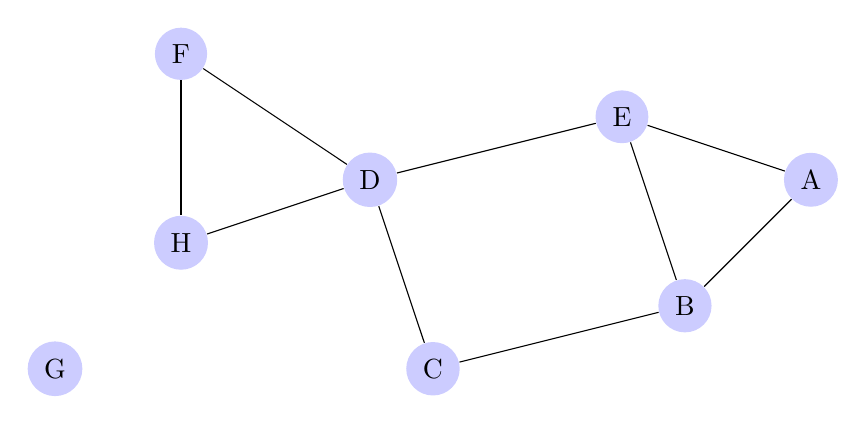
\begin{tikzpicture}
  [scale=.8,auto=left,every node/.style={circle,fill=blue!20}]
  \node (n6) at (1,10) {F};
  \node (n4) at (4,8)  {D};
  \node (n5) at (8,9)  {E};
  \node (n1) at (11,8) {A};
  \node (n2) at (9,6)  {B};
  \node (n3) at (5,5)  {C};
  \node (n7) at (-1,5)  {G};
  \node (n8) at (1,7)  {H};
  \foreach \from/\to in {n6/n4,n4/n5,n5/n1,n1/n2,n2/n5,n2/n3,n3/n4,n8/n4,n8/n6}
    \draw (\from) -- (\to);
\end{tikzpicture}
\end{center}
\inGerman{Person G hat gerade RetroShare installiert und noch keinen Freund. Person E ist mit A, B und D befreundet u.s.w.}
\inEnglish{User G has installed RetroShare just this minute and not yet added friends. User E ist friends with A, B und D and so forth...}

\inGerman{Im folgenden sei ein \underline{Freund} jeweils eine direkt mit dir befreundete Person, ein \underline{Freundesfreund} ein Freund einer deiner Freunde, mit dem du nicht befreundet bist. Wenn du z.B. die Person A wärst, wären deine Freunde E und B, deine Freundesfreunde C und D, und F bzw. H wären dann \underline{Freunde dritter Stufe}.}
\inEnglish{We shall call below ``a friend'' a person, which you have added as friend. A ``friend second grade'' shall be a friend of a friend of yours, with whom you are not friends. If f.e. you are person A, your friends would be E,B, your friends second grade would be C and D and the users F and H would be friends third grade to you.}

\inGerman{\emph{RetroShare verbindet sich ausschließlich mit direkten Freunden}, nicht mit Freundesfreunden.
Daher ist die Nutzung von RetroShare zu 100\% sicher, wenn man seinen Freunden vertrauen kann.
Eine kleine Ausnahme davon ist - falls eingeschaltet - das DHT, dazu im nächsten Abschnitt mehr.}
\inEnglish{\emph{RetroShare connects ONLY to your direct friends}, but not to your friends second or higher grade. So if you're adding only thrustworthy persons, you can be 100\% safe. The only (and small) exception to this rule is the DHT, see below for details.}

\inGerman{Person G kann RetroShare nicht benutzen, da er keine Freunde hat.
Würde nun D offline gehen, so würde sich dieses Netzwerk in zwei Unternetzwerke aufteilen, und somit wäre z.B. ein Dateitransfer zwischen H und A unmöglich.}
\inEnglish{So, a basic consequence is that G can't use RetroShare, because he has no friends.
If user D goes offline, the above RetroShare-network will split in two subnetworks and no communication or file transfer is possible between H and A anymore.}

\subsection{\inGerman{Verbindung zu Freunden}
\inEnglish{Connection with friends}} 
\inGerman{Die meisten Personen haben privat daheim keine statische IP Adresse, sondern eine sogenannte dynamische, die sich regelmäßig (meist alle 24h) ändert.
Das Problem dabei ist, dass RetroShare auch in der Lage sein muss, sich zu verbinden, wenn du und dein Freund beide für länger als 24h offline wart.
Dazu verwendet RetroShare je nach Einstellung bis zu drei verschiedene Methoden, die in den folgenden Unterkapiteln erklärt werden sollen.}
\inEnglish{Most people don't have a static ip address at home, instead they have a so called dynamic IP, which changes every 24 hours.
This is a problem, as RetroShare should be able to connect to your friend, if you and your friend are offline for more than 24 hours.
To get the IP address of your friend, RetroShare uses three different methods, which should be explained in the following subsections.}

\inGerman{Ich persönlich habe immer DHT und Discovery an, beides auszuschalten ist nur nötig, wenn die Benutzung von RetroShare selbst illegal wäre, wie vermutlich z.B. in China.}
\inEnglish{Personally, I've always DHT and Discovery activated, because deactivating both will make connections more complicated and I don't need to hide I'm using RetroShare, because I live in a free country.}

\subsubsection{DHT} \label{dht}
\inGerman{Das ``Distributed Hash Table'' ist die einfachste und bequemste Methode.
Dabei nutzt RetroShare momentan noch das ``Bittorrent-DHT'', das wohl größte weltweit.
Beachte, dass sich RetroShare hier ausnahmsweise auch mit dritten verbindet, allerdings nur um die IP-Adressen deiner Freunde nachzuschlagen.}
\inEnglish{The "Distributed Hash Table" is the easiest and comfortablest method.
RetroShare uses the "Bittorrent-DHT", the probably biggest world wide.
You should know, that RetroShare will make connections to strangers here, but ONLY to look up the IP-adresses of your friends.}

\inGerman{RetroShare wird dort in diesem verteilten Netzwerk einen Eintrag der Form (SSL-ID, IP-Adresse)  erzeugen.
Damit kann dann jeder, der deine SSL-ID kennt (deine Freunde und wenn du Discovery aktiviert hast, deine Freundesfreunde), deine IP Adresse bestimmen.
Wer deine SSL-ID nicht kennt, weiß nur, dass hinter deiner IP-Adresse ein RetroShare Nutzer steckt, mehr aber auch nicht, insbesondere nicht deinen RetroShare-Namen.}
\inEnglish{RetroShare will create an entry in this distributed network, which has the format (your SSLID, IP-adress).
Everyone, who knows your SSL-ID (your friends and - if you have Discovery turned on - your friends of friends), can determine your IP-Adress then.
People, who don't know your IP-adress, can only determine, that someone behind this IP is using RetroShare, but not the RetroShare nick, which friends he has or what he does.}

\inGerman{Wer das DHT nicht aktiviert, dem sei dringend die Einrichtung einer dynamischen DNS empfohlen, siehe weiter unten.}
\inEnglish{If you don't want to make public, that your IP is using RetroShare, and you want to turn it off, you should setup Dynamic DNS, see section \ref{dyndns}.}

\inGerman{Das DHT stellt mit vielen Personen gleichzeitig eine Verbindung her, was manche Router nicht vertragen zu scheinen.
Dies äußert sich in ständigen Verbindungsabbrüchen zu deinen Freunden.}
\inEnglish{The DHT makes a bunch of connections at the same time, and some consumer routers don't like that.
This results in connection losses every five minutes or so.}

\subsubsection{Discovery} \label{discovery}
\inGerman{Bei Discovery erlaubst du deinen Freunden, deinen Schl\"ussel und deine IP an deren Freunde weiterzugeben, d.h. an deine Freunde zweiter Stufe.
Zudem teilst du allen deinen Freunden mit, mit wem du befreundet bist.
Dies hat zwei Folgen:}
\inEnglish{With Discovery turned on, you allow your friends, to give your key and your IP to all of their friends, i.e. to your friends of second grade.
Moreover, you send your friendlist to all of your friends.
This implies two things:}
\begin{itemize}
\item
\inGerman{\emph{Zu dir kann leichter verbunden werden.}
Stell dir vor, du bist im obigen Netzwerk F und du bist mit D verbunden bist, H ist offline.
Nun kommt H online, weiss aber zun\"achst nur die IP von D und verbindet sich mit diesem.
Wenn du Discovery an hast, wird nun D deine IP an H schicken, und H kann sich zu dir verbinden.}
\inEnglish{\emph{It's easier to connect to you.}
Imagine, you are F in the network above and you're currently connected to D, H is offline.
Now H goes online, but knows only the IP of D and connects to him.
If you have discovery on, D now will send your IP to H and H can connect to you.}
\item
\inGerman{\emph{Es ist einfacher, mit dir Freund zu werden.}
Angenommen, du bist wieder F und du und E m\"ochten nun Freunde werden.
Wenn du Discovery an hast, hat E nun schon deinen Schl\"ussel von deinem Freund D geschickt bekommen, und somit ist das Adden nun nur noch ein Mausklick.
Der umst\"andliche Austausch von Zertifikaten ist nun nicht mehr n\"otig.}
\inEnglish{\emph{It is easier, to become friends with you, if you want to.}
Imagine, you're F again, and you and E want to be friends now.
If you have Discovery turned on, E will already have your key (your common friend D has sent your key) and adding friends is only a mouseclick anymore.
The annoying manual key exchange is no longer necessary.
}
\end{itemize}

\subsubsection{DynDNS} \label{dyndns}
\inGerman{Die wohl beste Methode ist es, dass du selbst eine sogenannte ``dynamische DNS'' einrichtest.
Dazu kannst du z.B. auf der Seite \url{http://no-ip.org} oder diversen anderen eine dynamische DNS der Form ``irgendwas.no-ip.org'' registrieren und diese von deinem PC oder am besten sogar deinem Router direkt aktualisieren lassen, falls sie sich geändert hat.}
\inEnglish{The best method to increase your connectivity is the setup of "dynamic DNS".
You need to go to a site like \url{http://no-ip.org} and register a dyndns like "something.no-ip.org".
This DNS entry can be updated from your PC regularly or (even better) directly by your router.}

\inGerman{Das Einrichten einer dynamischen DNS soll hier nicht weiter erklärt werden, da es den Rahmen sprengt.}
\inEnglish{The setup of dynamic DNS is beyond the scope of this document, just google it.}

\inGerman{Deine Freunde bzw. deren RetroShare kann dann einfach die DNS ``irgendwas.no-ip.org'' nachschlagen und kann deine IP-Adresse sofort ermitteln.}
\inEnglish{Your friends (resp. their RetroShare) can then make a simple DNS query and will get your current IP.}

\inGerman{Mit einer funktionierenden DynDNS Einrichtung kann DHT und Discovery ausgeschaltet werden.}
\inEnglish{With a working DynDNS setup, you can disable DHT and Discovery.}

\subsection{Chat}
\inGerman{RetroShare unterstützt Instant-Messaging mit direkten Freunden. Einfach in der Freundesliste auf den Namen doppelt klicken und das Chatfenster öffnet sich.}
\inEnglish{RetroShare allows Instant Messaging with your direct friends. Just doubleclick in the friends list on a name and the chat window opens.}
 
\inGerman{Nachrichten, die du deinem Freund schreibst, während er offline ist, werden erst zugestellt, wenn du und dein Freund wieder miteinander verbunden sind! Sie werden ja nicht wie üblich auf einem Server zwischengespeichert.}
\inEnglish{Beware: Messages, which your writing when your friend is offline, will be not be delivered until you and your friend are connected again! There is no central server, which could save the messages for you, as you might be used to. }

\subsection{\inGerman{Gruppenchat}\inEnglish{Group Chat}}
\inGerman{Im Gruppenchat können Nachrichten an alle Freunde, die online sind gesendet werden. Freunde, die gerade offline sind, erhalten diese nicht.}
\inEnglish{Using the group chat allows you to send a message to all of your direct friends which are online. Offline friends won't get the message, even if they get online later.}

\inGerman{Das f\"uhrt dazu, dass man im Gruppenchat nur ``Gespenst''-Chats mitlesen kann, d.h. nur die Nachrichten von einer Person. Denn unterhalten sich z.B. E und D im Gruppenchat, so kann die komplette Konversation nur von E und D mitgelesen werden, hingegen erhalten A und B nur die Nachrichten von E, und C,F,H können nur die Nachrichten von D lesen.}
\inEnglish{This has the consequence, that you'll notice ``ghost-chats'' in the group chat window sometimes, i.e. you can read only the messages of one person. For example, if E and D are chatting using the group chat, only those two can read both parts of the conversation. A and B will get only the messages from E, and C,F,H will only get D's messages.}

\inGerman{Der Gruppenchat ist meiner Meinung nach nur für Meldungen wie z.B. ``Ich bin die nächsten 4 Tage offline.'' etc. nützlich.}
\inEnglish{The group chat is probably not the most useful feature, I use it only for messages like ``I'm offline the next week.''.}

\subsection{\inGerman{Nachrichten}\inEnglish{Messages}}
\inGerman{Ähnlich wie der Chat funktioniert auch das Versenden von Nachrichten. Diese können nur zugestellt werden, wenn der Empfänger zur selben Zeit wie du online ist.
Falls also A an B eine Nachricht schreibt, aber A immer nur von 8 bis 12 Uhr online ist, B hingegen nur von 13-18 Uhr, so wird diese Nachricht niemals zugestellt werden.}
\inEnglish{The delivery of messages is similar to the delivery of chat messages. They will only be delivered, if you and your friend are connected, otherwise the messages will stay in the outbox. So, if A is writing a message to B, but A is online only from 8am to 12am, B instead only from 1pm to 6pm, the message will never be delivered.}

\subsection{\inGerman{Datei Transfer}\inEnglish{File Transfer}} \label{filetransfer}

\inGerman{Das fortgeschrittenste Feature an RetroShare ist wohl der Austausch von Dateien. Bei der Freigabe von Dateien gibt es drei Möglichkeiten, wie die Dateien freigegeben werden sollen, nämlich
\begin{itemize}
 \item netzwerkweit
 \item durchsuchbar von Freunden
 \item durchsuchbar von ein oder mehreren Gruppen von Freunden
\end{itemize}
Es macht natürlich keinen Sinn, in RetroShare Dateien freizugeben ohne mindestens eine der drei Freigabetypen auszuwählen, da die Dateien sonst gar nicht wirklich freigeben werden.
Was genau die beiden Freigabetypen bedeuten, soll in den beiden folgenden Unterkapiteln behandelt werden.}
\inEnglish{Probably the most advanced feature of RetroShare is the exchange of files. Everyone can share one or more folders, and there are the following three options:
\begin{itemize}
 \item networkwide
 \item browsable by friends
 \item browsable only by a group of friends
\end{itemize}
Of course, it is pointless to adding a folder, without at least one of those options enabled. 
What those options mean, will be explained in the next chapters.}

\subsubsection{\inGerman{durchsuchbare Freigaben}\inEnglish{browsable by friends}}
\inGerman{Diese Art von Freigabe eignet sich am besten für private Dateien, wie z.B. Urlaubsfotos. Alle direkten Freunde von dir sehen diese Dateien in ihrem ``Dateien'' Fenster und können dort das Herunterladen in Auftrag geben.}
\inEnglish{This option allows all your direct friends to see and browse this folder in their ``Files'' Tab. They can download then the complete folder or some parts of it.}

\inGerman{Sobald sie dies tun, wirst du diese Dateien in deinem Upload Fenster sehen und dort auch den Namen des Freundes, der diese herunterlädt. Auch der Freund sieht deinen Namen als Quelle der Datei, die er herunterlädt.}
\inEnglish{As soon as your friend starts downloading some browsable shared files, you'll see his name and the file in the upload window.}

\inGerman{Insbesondere weiß jeder deiner Freunde, dass du diese Datei freigegeben hast.}
\inEnglish{Noteworthy is, that all your friends will know that these files are from you.}

\subsubsection{\inGerman{Anonyme Freigaben}\inEnglish{Anonymous shares}}
\inGerman{Diese Art von Freigabe eignet sich dazu, dass nicht einmal Freunde sicher wissen können, was du freigegeben hast.}
\inEnglish{This option of sharing a folder allows you to share files, without your friends knowing it.}

\inGerman{In diesem Abschnitt seist du Person A aus obigem Graph, und du hast einen Ordner ``Test'' mit der Datei ``Testdatei'' nur anonym, nicht aber durchsuchbar freigegeben. Insbesondere taucht dieser Testordner nicht im Tab Dateien auf und kann nur \"ueber die Suche gefunden werden.}
\inEnglish{In this subsection, we'll assume that you are person A from the above graph, and you are sharing the folder ``Test'', which contains the file ``Testfile''. Nobody will see this folder in his ``Files'' tab then, it can only be found using the search function.}

\inGerman{Angenommen F sucht nun nach dem Begriff ``Testdatei''.
F schickt seine Suchanfrage nach D, D leitet die Suchanfrage weiter an E und C,  usw. und irgendwann landet die Suchanfrage bei dir und du meldest einen Treffer.
Jeder Knoten hat sich nun kurzzeitig gemerkt von wem er an wen die Suchanfrage weitergeleitet hat (z.B. merkt sich E: ``Ich habe die Suchanfrage nach ''Testdatei`` und der ID 128931 von D nach A weitergeleitet.'').
So ist es möglich, dass du deinen Treffer an F zurücksenden kannst, ohne dass irgendein Knoten sichere Information hat, wer gesucht und wer den Treffer hat.}
\inEnglish{Let's assume, that F searches for "Testfile".
F sends a search request to D, D forwards this request to E and C, and so on, and after a few hops, the search request arrives at you and you - having "Testfile" - send a hit back.
Every node has a temporary cache, from who he forwarded which search request to whom (e.g. E remembers: "I have forwarded the search request for "Testfile" with the ID 128931 from D to A).
This way, it is possible, that your success message can be sent the same way back to F, without any node between knowing who searched and who had the hit.}

\inGerman{So können ``Anonyme F2F Tunnel'' über maximal 6 Knoten aufgebaut werden und man kann auch Dateien netzwerkweit tauschen, ohne jemals Dateien an andere außer deinen Freunden zu senden.}
\inEnglish{This way, it is possible to establish "Anonymous F2F tunnels" up to a maximum of 6 hops and you can share files networkwide, without ever making a connection with other peers except your friends.}

\inGerman{Betrachten wir nun, was jeder Teilnehmer eines solchen ``Anonymer F2F-Tunnel'' weiß, am Beispiel des obigen Tunnels A $\leftrightarrow$ E $\leftrightarrow$ D  $\leftrightarrow$ F:
\begin{itemize}
 \item A weiß, dass er die Datei ``Testdatei'' an seinen Freund E hochlädt. (In der GUI wird im Upload Fenster nur ``Anonymer F2F-Tunnel'' angezeigt). Er weiß nicht, ob E diese Datei angefordert hat, oder E sie nur weiterleitet.
 \item E weiß nur, dass er eine Datei von A nach D weiterleitet. Er kann den Inhalt der Datei einsehen, weiß aber nicht, ob A sie hochlädt, oder E sie herunterlädt.
 \item Analog weiß D nur, dass er eine Datei von E nach F weiterleitet, könnte jedoch den Inhalt des weitergeleiteten anschauen.
 \item F weiß nur, dass er die Datei ``Testdatei'' von D herunterlädt. Er weiß nicht, ob D sie hochlädt oder nur weiterleitet.
\end{itemize}}
\inEnglish{Let's look at the information, each participant of this "Anonymous F2F-Tunnel" knows, looking at the example tunnel A $\leftrightarrow$ E $\leftrightarrow$ D  $\leftrightarrow$ F from above.
\begin{itemize}
\item A knows, that he is uploading the file "Testfile" to his friend E. (In the GUI, he'll see as Peer only "Anonymous F2F-Tunnel"). He doesn't know, if E requests this file, or E forwards this file.
\item E knows, that he forwards a file from A to D. He could spy on what he is transferring, but he can't say, if A is uploading the file or E is downloading it. They could both forward this file from someone else.
\item Analogue, D knows, he's forwarding a file from E to F and he could look at the file.
\item F knows, that he is downloading the file "Testfile" from D, but he doesn't know, if D shares this file, or is just forwarding it.
\end{itemize}}

\inGerman{Natürlich wird die Downloadgeschwindigkeit bei längeren Tunneln meist recht langsam sein, hängt sie doch vom ``schwächsten'' Glied der Kette ab. 
Hat z.B. E nur einen sehr langsamen Internetanschluss, so wird die Verbindung zwischen F und A auch sehr langsam sein.}
\inEnglish{Of course, the download speed of a long tunnel will most of the time be very slow, because it depends on the weakest link in the chain.
If e.g. E has only a very slow internet connection, tunnels between F and A will be slow, too.}

\inGerman{Die Nachteile an anonymen Freigaben sind, dass diese nur über die Suche gefunden werden können und zudem nicht das Tauschen in Ordnerstrukturen erlauben.
Möchte man nun trotzdem einen kompletten Ordner dem gesamten RetroShare Netzwerk komfortabel zum Download anbieten, so ist die beste Methode, für diesen Ordner eine Kollektion (siehe \ref{rscollection}) zu erstellen und anschließend den RetroShare-Link zu dieser ``.rscollection''-Datei in einem Forum zu posten.}
\inEnglish{The downsides of anonymous shares are, that other people can find those only by using the search and that they don't allow sharing complete folders.
If you want to share a complete folder with the whole network anyway, the best way is, to create a collection (see section \ref{rscollection}) and then post the link to this collection file anonymously in a forum.}
 
\inGerman{Genauere technische Details gibt es in der offiziellen Dokumentation \url{http://retroshare.sourceforge.net/wiki/index.php/Documentation:TurtleHopping}.}
\inEnglish{More about technical details can be read at the official documentation \url{http://retroshare.sourceforge.net/wiki/index.php/Documentation:TurtleHopping}.}

\subsubsection{Swarming}
\inGerman{RetroShare unterstützt das Torrent-Prinzip, d.h. jeder, der eine Datei herunterlädt, kann diese im selben Moment schon wieder hochladen.
Auch der Download von mehreren Quellen gleichzeitig ist möglich.}
\inEnglish{RetroShare is capable of the so called "swarming", i.e. everyone, who downloads a file, can upload this at the same moment without having the complete file.
The download from multiple sources is possible, too.}

\inGerman{Jede Datei wird dazu in Blöcke von 1MB geteilt und ausschließlich über den Hash der Datei identifiziert, d.h. haben zwei User dieselbe Datei mit anderem Namen, so kann ein dritter User trotzdem von beiden diese Datei herunterladen.}
\inEnglish{Every file is divided into chunks of 1MB and the file is only identified by the hash, i.e. if two users have the same file with different names, a third user can still download from both of them.}

\subsubsection{RetroShare-Links}

\inGerman{RetroShare-intern können Links zu Dateien verbreitet werden. Ein Beispiel-Link wäre}
\inEnglish{There exists RetroShare-internal links to files. A example link is:}

retroshare://file?{\color{green}name=RSCounterFile.txt}\&{\color{yellow}size=200}\&{\color{red}hash=d89f3b4f3fe842ac9164fb19b8d1ab6b2e238d61}

\inGerman{Man sieht, dass dieser nur aus den folgenden Komponenten besteht:
\begin{itemize}
 \item {\color{green}Dateinamen}: Dieser teilt RetroShare mit, unter welchem Namen es die Datei nach dem Download abspeichern soll. Dieser kann beliebig verändert werden, der Link funktioniert trotzdem noch.
 \item {\color{yellow}Dateigröße}: RetroShare muss die Größe der Datei wissen.
 \item {\color{red}Hash}: Über den Hash identifiziert RetroShare, welche Datei es herunterladen soll. Es ist dabei sehr, sehr unwahrscheinlich, dass zwei Dateien weltweit denselben Hash haben.
\end{itemize}}
\inEnglish{You can see, that such a link consists only of the following components:
\begin{itemize}
\item {\color{green}the file name}: This name is the name, RetroShare saves the file to. It can be modified arbitrarily and the link is still valid.
\item {\color{yellow}file size}: RetroShare needs to know, how big the file is.
\item {\color{red}Hash}: The SHA1 hash of the file is used, to identify which file should be downloaded. It's very very unlikely, that two files worldwide have the same hash.
\end{itemize}}

\subsubsection{\inGerman{RetroShare-Kollektionen}\inEnglish{RetroShare-Collections}} \label{rscollection}

\inGerman{Mittels ``.rscollection''-Dateien können auch komplette Ordner samt Unterordner und allen enthaltenen Dateien bequem heruntergeladen werden.
Eine RSCollection ist dabei nur eine Datei mit der Endung ``.rscollection''.
Es handelt sich dabei um eine XML-Datei, sie enthält eine Ordnerhierarchie und die dazugehörigen Hashs.
Ein Beispiel für den Inhalt einer Collection-Datei wäre:}
\inEnglish{With ".rscollection" files, complete folders with subfolders and all contained files can easiliy be downloaded.
A collection is simply a XML file, which contains the folder structure and all names/hashes of the files.
An example collection looks like this:}

\begin{lstlisting}
<!DOCTYPE RsCollection>
<RsCollection>
 <Directory name="Mainfolder">
  <File size="100" sha1="23f744d9b68841f31e4fe24473066a794898a5bc" name="file1.txt"/>
  <File size="100" sha1="5f695778740e9f7f63022083f62a09ecc07aaa35" name="file2.txt"/>
  <Directory name="Subfolder">
   <File size="200" sha1="2cc55a96942996e1cf870ee43bb269a5cd57d342" name="file3.txt"/>
   <File size="200" sha1="e84e958c18b2fa3e2014c347f7e974e2b797523f" name="file4.txt"/>
  </Directory>
 </Directory>
</RsCollection>
\end{lstlisting}
\inGerman{Diese 4 Dateien in dieser RSCollection k\"onnten nun heruntergeladen werden, indem diese Kollektion mittels des Buttons "Oeffne Kollektion" im Transfers-Fenster geoeffnet wird. 
Dadurch wird zuerst im eingehenden Ordner zuerst die richtige Ordnerstruktur erstellt (im Beispiel die Ordner "incoming/Hauptordner" und "incoming/Hauptordner/Unterordner") und anschließend alle ausgewählten Dateien zum Download in Auftrag gegeben.
Nachdem der Download einer Datei abgeschlossen ist, wird diese automatisch in den passenden Unterordner kopiert.}
\inEnglish{These 4 files of this RSCollection can now be downloaded by using the button "Open Collection" in the Transfers-tab.
If you do this, RetroShare will create the folder structure for you (in the example the folders "incoming/Mainfolder" and "incoming/Mainfolder/Subfolder") and then queue all 4 files in the download queue.
After finishing the download of one of those 4 files, it'll be moved into the correct subfolder automatically.}

\subsection{Foren} \label{foren}

\inGerman{Foren erlauben den dezentralen Austausch von Nachrichten mit beliebig weit entfernten Teilnehmern des Netzwerkes. Jeder Teilnehmer kann ein Forum erstellen, dieses Forum sehen dann zunächst alle Freunde des Erstellers.}
\inEnglish{}

\inGerman{Foren verbreiten sich nur weiter, indem jemand sie abonniert. Dies dient dazu, dass Spam verhindert wird. Jeder, der ein Forum abonniert, verbreitet dieses an alle seine Freunde weiter. So gesehen ist das Abonnieren eines Forums auch eine Empfehlung dieses Forums an deine Freunde. Das Schreiben von Artikeln in Foren ist nur möglich, falls man dieses Forum abonniert hat.}
\inEnglish{}

\inGerman{Foren können nur gelöscht werden, indem jede Person das Abonnement kündigt. Solange noch eine Person das Forum abonniert hat, ist dieses auch noch im Netzwerk verfügbar. Du kannst also auch bei selbsterstellten Foren das Abonnement kündigen.}
\inEnglish{}

\inGerman{Im Beispiel funktioniert das so: Erstellt A ein Forum, so können es also A, B, D sehen. Abonniert B noch zusätzlich dieses Forum, so können es nun A, B, C, E sehen. Möchte A nun das Forum löschen, so kann er diesem das Abonnement kündigen, jedoch wird das Forum trotzdem noch für B und dessen Freunde sichtbar bleiben (also A, B, C, E), bis auch B sich austrägt und das Forum endgültig nicht weiter verteilt wird. Bei allen Leuten, die dieses Forum jedoch einmal gesehen haben (hier A,B,C,E), bleiben die Nachrichten momentan im Cache und somit für alle Zeit erhalten.}
\inEnglish{}

\inGerman{In der momentanen Implementation verschwinden Foreneintr\"age nach gut einem Jahr.}
\inEnglish{With the current implementation, RetroShare discards forum messages after some more after a year.}

\subsubsection{\inGerman{AUTHentifizierte Foren}\inEnglish{AUTHenticated Forums}}
\inGerman{Bei authentifizierten Foren wird für jede Nachricht eine gültige Unterschrift verlangt.
Somit ist einsehbar, welcher Person (genauer welcher PGP Schlüssel) diese Nachricht erstellt hat.}
\inEnglish{If a forum is Authenticated, a signature is required for each message.
This ensures, that everybody knows, which person (more precisely which PGP key), created this message.}

\inGerman{Falls die Unterschrift nicht verifiziert werden kann, da der PGP-Schlüssel mit der passenden ID nicht bekannt ist (z.B. Nachricht von jemanden, der weder Freund noch Freundesfreund von dir ist), so wird hier eine ``Fehlende Nachricht'' angezeigt.
Somit sind von dir geschriebene Nachrichten auch maximal von Freundesfreunden lesbar und Nachrichten verbreiten sich nicht beliebig weit im RetroShare-Netzwerk.}
\inEnglish{If the signature can't be verified by your RetroShare, because the PGP-key with the related ID is not known (e.g. a message from someone, which is a friend of third or more grade), this message won't be displayed.
This has the consequence, that you can read only messages from friends or friends of second grade.
You'll get the other messages, too, but the current implementation won't display it.}

\subsubsection{\inGerman{Anonyme Foren}\inEnglish{Anonymous Forums}}
\inGerman{Bei authentifizierten Nachrichten ist keine Unterschrift erforderlich und somit kann jeder anonym schreiben.
Nachrichten verbreiten sich beliebig weit, und niemand weiß, wer eine Nachricht geschrieben hat.}
\inEnglish{In anonymous forums no signature is required and everyone can post anonymously.
Thus, messages distribute infinitely far and can be read by everyone, who can read this forum.}

\inGerman{Optional kann man seine Nachrichten trotzdem unterschreiben, damit den anderen klar wird, dass die Nachricht in dem anonymen Forum auch wirklich von dir stammt. Somit kann auch in anonymen Foren ein Nachweis erbracht werden, wer die Nachricht geschrieben hat.}
\inEnglish{You can - if you want to - still sign the messages, so everyone with your key knows, that the message is from you. This makes it even in anonymous forums possible to prove that a certain message is from a certain person.}

\subsection{\inGerman{Kanäle}\inEnglish{Channels}}
\inGerman{Ein Kanal ermöglicht es einer Person neue Nachrichten bzw. Dateien RetroShare-intern zu veröffentlichen.
Ich sehe in meiner Liste z.B. einen Kanal mit aktuellen Versionen von RetroShare als auch einen Kanal mit IT-News.}
\inEnglish{A channels allows a person to spread new messages or files. I can see e.g. a channel with current RetroShare builds as well as a channel with IT-News.}

\inGerman{Die Sichtbarkeit von Kanälen ist dabei genauso wie die Sichtbarkeit von Foren, für Details siehe dazu das Kapitel \ref{foren}.}
\inEnglish{}

\inGerman{Für jeden Kanal wird ein GnuPG-Schlüssel erzeugt. Jeder der den privaten Schlüssel dieses Kanals besitzt kann dort neue Nachrichten schreiben. Bei der Erstellung kann man auswählen, ob nur man selbst oder einige ausgewählte Personen diesen privaten Schlüssel erhalten und somit veröffentlichen können (Regelfall) oder jede Person (nicht besonders nützlich meiner Meinung nach).}
\inEnglish{}

\inGerman{Das Abonnieren eines Kanals führt dazu, dass dort veröffentliche Dateien automatisch heruntergeladen werden, dies kann jedoch auch deaktiviert werden.}
\inEnglish{}

\subsection{Chatlobbies}
\inGerman{Chatlobbies ermöglichen es auch mit nicht befreundeten Personen dezentral zu chatten. Im Beispiel oben könnten somit F, D, E und A miteinander chatten.}
\inEnglish{}

\inGerman{Bei Chatlobbies findet niemals eine Authentifizierung statt, jeder kann sich mit einem beliebigen Namen in der Chatlobby anmelden!
Seinen Nicknamen kann man in den Optionen im Unterpunkt ``Chat'' ändern.
Insbesondere könnte Person A als Nicknamen auch ``Person B'' wählen und somit sich als jemand anderes ausgeben!}
\inEnglish{}

\inGerman{Es gibt sowohl öffentliche Chatlobbies, die jeder Nutzer sieht, als auch private, die man nur nach Einladung eines Mitglieds sieht.}
\inEnglish{}

\inGerman{Genaue technische Details findet man auf der offiziellen Dokumentationsseite \url{http://retroshare.sourceforge.net/wiki/index.php/Documentation:ChatLobbies}.}
\inEnglish{}

\subsubsection{private Chatlobbies}
\inGerman{Private Chatlobbies sieht man nur, indem man eine Einladung dazu erhält. Leider sind private Chatlobbies zur Zeit etwas benutzerunfreundlich, denn started man RetroShare neu, so muss man von einem Mitglied, dass noch in der privaten Chatlobby ist, wieder neu eingeladen werden.}
\inEnglish{}

\subsubsection{öffentliche Chatlobbies}
\inGerman{Ist mindestens ein Freund von dir in einer öffentlichen Chatlobby eingeloggt, so siehst du diese auch und kannst ebenfalls beitreten. Die Sichtbarkeit ist also wieder wie bei den Foren, vgl. Abschnitt \ref{foren}.}
\inEnglish{}

\subsection{Relays}
\inGerman{RetroShare stellt eine Methode bereit, mit dem ein technisch versierterer Freund anderen Nutzern die Verbindung ins Retrosharenetz ermöglicht, sofern diese keinerlei Einfluss auf ihre Netzwerkgebenheiten haben.}
\inEnglish{}

\inGerman{Bei manchen Internetanbindungen ermöglichen äußere Umstände keine Benutzung des DHT.
Ein anderer RetroShare-Benutzer kann mittels der Relay Optionen jeweils für Freunde, Freundesfreunde oder sonstige Bandbreite reservieren, durch den der DHT Traffic geleitet werden kann.
Somit ist auch für Leute hinter einer Firewall eine Benutzung des DHTs möglich.}
\inEnglish{}

\inGerman{Um Missverständnissen zu vermeiden:
Relays sind nicht dazu gedacht, den Upload für seine Freunde und Freundesfreunde zu steuern!
Vielmehr bieten Relays die Möglichkeit auch in geschlossenen Systemen (Firmennetzwerk, vom ISP geblocktes DHT (z.b. in China)), über eine oder mehrere Relay-Verbindung zu Freunden eine Verbindung zum Retrosharenetzwerkt zu erhalten.}
\inEnglish{}

\inGerman{Stellt man selbst eine Relay-Verbindung zur Verfügung und reserviert Bandbreite für diese, so sollte man beachten, dass diese Bandbreite vom Download und vom Upload gleichermaßen abgezogen wird.
Sofern man selbst keine Relay-Verbindung benötigt und Freunde nicht auf diese angewiesen sind, kann Relay in den Optionen standartmäßig deaktiviert werden.}
\inEnglish{}

\newpage
\section{\inGerman{H\"aufig gestellte Fragen (FAQ)}
\inEnglish{Frequently asked questions}}
%
\inGerman{Die offizielle FAQ auf englisch befindet sich unter \url{http://retroshare.sourceforge.net/wiki/index.php/Frequently_Asked_Questions}.
Einige häufig gestellten Fragen möchten wir auch hier beantworten.}
\inEnglish{The official FAQs can be found at \url{http://retroshare.sourceforge.net/wiki/index.php/Frequently_Asked_Questions}.
Some questions we'll answer here, too.}

\subsection{\inGerman{Allgemeines}
\inEnglish{General}}

\subsubsection{\inGerman{Windows: Was ist der Unterschied zwischen der installierbaren und der portablen Retroshare Version}
\inEnglish{Windows: What's the difference between fixed and portable Installation?}}
%
\inGerman{Die installierbare Version kommt mit einem Installer und speichert die Profile in \%appdata\%/RetroShare.
Die portable Version besteht aus einer einzigen Datei RetroShare.exe, und speichert s\"amtliche Dateien in einem Ordner.
Empfehlenswert ist es die portable Version zu verwenden, da sich diese einfacher updaten lässt.}
\inEnglish{\todo{write}}

\subsubsection{\inGerman{Wie update ich mein Retroshare Portable?}
\inEnglish{How can I update RetroShare?}}
\todo{write}

\subsubsection{\inGerman{Windows: Wie wechsele ich von einer bestehenden Retroshare Installation auf Retroshare Portable?}
\inEnglish{Windows: How can I move my current fixed RetroShare Installation to a portable one?}}
\todo{write}

\subsubsection{\inGerman{Ist es möglich Retroshare auf mehreren Rechnern mit dem gleichen Identität zu betreiben?}
\inEnglish{Is it possible, to run RetroShare on multiple devices with the same identity?}}
%
\inGerman{Ja, dafür sind die sogenannten Locations vorgesehen.
1) ProfilManger aufrufen: Freunde -> Profil --> Profilmanager
2) Eigene Identität exportieren
3) Auf anderem Rechner die frische RS Portable starten und das bei 2) erstellte Identität importieren
4) Jetzt sollte man erstmal die beiden Identitäten miteinander befreunden (wie gewohnt keys tauschen)
5) Da man mit der neuen Identität noch nicht automatisch seine Freundesliste bekommt, empfiehlt es sich momentan noch von der alten Identität eine Freundesempfehlung mit allen Freunden an die neue Identität zu schicken.}
\inEnglish{\todo{write}}

\subsubsection{\inGerman{Kann man Ordnerfreigaben nur für bestimmte Gruppen / Personen Freigeben?}
\inEnglish{Is it possible to share files only with a certain group of friends?}}
\todo{write: yes, and soon even for anonymous shares}

\subsubsection{\inGerman{Warum ist RetroShare so träge, besonders nach dem Starten?}
\inEnglish{Why is RetroShare so slow, especially on startup?}}
\inGerman{Die aktuelle Version von RetroShare überprüft beim Start jedesmal alle Signaturen von Forennachrichten, Channelnachrichten u.v.m. Dies dauert je nach Größe deines Netzwerkes bis zu 15min mit hoher CPU-Last und sehr trägem Verhalten von RetroShare. Danach läuft es jedoch sehr stabil und mit geringer CPU-Last.}
\inGerman{Dieses unsinnige Verhalten wird wohl von den Entwicklern in einer späteren Version behoben werden.}
\inEnglish{\todo{write}}


\subsubsection{\inGerman{Wie ist RetroShare lizenziert?}
\inEnglish{How is RetroShare licenced?}}
\inGerman{RetroShare ist Open Source, d.h. jeder weltweit kann den Quelltext herunterladen und nachvollziehen, wie RetroShare funktioniert.
Die einzelnen Teile von RetroShare sind dabei laut Angabe der Entwickler folgendermaßen lizenziert:}
\begin{itemize}
 \item openSSL: BSD style
 \item KadC: GPL + exception (asked author for exception)
 \item threads: LGPL
 \item RetroShare Library: LGPL
 \item RetroShare GUI + QT: GPL + exception
\end{itemize}
\inEnglish{\todo{improve}}

\subsubsection{\inGerman{Ich muss meinen Computer neu installieren. Wie sichere ich meine RetroShare Installation?}
\inEnglish{I have to reinstall my computer. What do I have to backup?}}
%
\inGerman{Es müssen zwei Dinge gesichert werden, die Daten von GnuPG und die von RetroShare. Unter Linux genügt es, im Home-Ordner die versteckten Ordner ``.pgp'' und ``.retroshare'' zu sichern und diese nach der Neuinstallation zurückzukopieren. \todo{Windows}}
\inEnglish{\todo{write}}

\subsubsection{\inGerman{Warum benutzt RetroShare soviel Bandbreite, obwohl ich nichts freigegeben habe und auch nichts herunterlade?}
\inEnglish{Why does RetroShare use so much bandwidth, although I'm not up- or downloading anything?}}
\inGerman{Wahrscheinlich hast du gerade viel ``F2F-Transfer'', d.h. du leitest Dateien von einem Freund zum anderen weiter. 
Für Details siehe dazu auch den Abschnitt \ref{dateitransfer}.}
\inEnglish{write F2F tunnel transfer}

\subsubsection{\inGerman{Gibt es eine Obergrenze von Freunden?}
\inEnglish{Is there a maximum number of friends I can add?}}
\inGerman{Einge User beklagen, dass RetroShare bei extrem vielen Freunden (so um die 150 Stück) zu Verbindungsabbrüchen neigt. Man sollte es also (noch) nicht übertreiben. Die Obergrenze hängt u.a. auch von des verwendeten Router und der verfügbaren Internet-Bandbreite ab. Je schneller die Verbindung desdo mehr Freunde sind momentan möglich. Es ist zu erwarten, dass die Obergrenze mit der Einführung des neuen Cache-Systems weiter steigt.}
\inEnglish{\todo{write}}


\subsubsection{\inGerman{Wie viele Leute benutzen RetroShare?}
\inEnglish{How many people are already using RetroShare?}}
\inGerman{Das kann nicht mit Sicherheit gesagt werden, da RetroShare im ``Darknet''-Modus keinerlei Spuren im Internet hinterlässt.
Nach (unzuverlässigen) Schätzungen, die auf dem DHT beruhen, sind wohl weltweit immer um die 1000 User gleichzeitig online.
Ob diese alle im selben Netzwerk sind, kann jedoch nicht gesagt werden.}
\inEnglish{\todo{write: impossible, but 1000 acc. to DHT}}

\subsubsection{\inGerman{Was sind Cache-Transfers? Was bedeuten die fc-own bzw. grp-*.dist Dateien im Transfer-Fenster?}
\inEnglish{What are Cache-Transfers? What are the fc-own resp. grp-*.dist files in the Transfer-Tab?}}
\inGerman{In Cache-Transfers sind die Foren und Channel Nachrichten (grp-*.dist) als auch die Listen von durchsuchbar freigegebenen Dateien (fc-own.rsfb) enthalten.}
\inEnglish{\todo{write}}

\subsubsection{\inGerman{Warum brechen meine Verbindungen mit Freunden ständig ab (Freund geht offline und gleich wieder online)?}
\inEnglish{Why are the connections to my friends so unstable (friend is going off- and online often)?}}
\inGerman{Stelle sicher, dass dein Port weitergeleitet ist, z.B. mithilfe der Seite \url{http://canyouseeme.org}.
Falls der Port weitergeleitet ist, könnte es auch daran liegen, dass dein Router die vielen gleichzeitigen Verbindungen des DHT (Abschnitt \ref{dht}) nicht verträgt.
Unter Optionen->server->netzwerkkonfiguration kann DHT ausgeschaltet werden.
Zudem koennte es daran liegen, dass die CPU Auslastung zu hoch ist und daher die Verbindungen abbrechen.}
\inEnglish{\todo{write: port forward, router DHT problem, too many friends}}

\subsubsection{\inGerman{Warum funktioniert DHT nicht mehr? Warum bleibt DHT rot und NAT nur gelb, obwohl ich meinen Port definitiv weitergeleitet habe?}
\inEnglish{Why doesn't DHT work anymore? Why does the DHT icon stay red and the NAT icon stay yellow, although I forwarded my port?}}
\inGerman{Dies liegt meist an einem der folgenden Gründe:
\begin{itemize}
\item Port von RetroShare ist nicht weitergeleitet. Überprüfe dies z.B. mit \url{http://www.canyouseeme.org}.
\item RetroShare wird durch die Firewall des Rechners blockiert.
\item Durch einen Crash von RetroShare wurde die Datei bdboot.txt im Konfigurationsverzeichnis beschädigt (meist leer). Sie enthät die Startknoten für das DHT (siehe \ref{dht}) und darf nicht leer sein. Abhilfe schafft meist ein simples Löschen dieser Datei, dann wird RetroShare diese beim nächsten Start mit einer mitgelieferten Standard Version überschreiben.
\end{itemize}}
\inEnglish{\todo{write: port, firewall, empty bdboot.txt}}

\subsubsection{\inGerman{Warum ist der Download so langsam?}
\inEnglish{Why is the download of files so slow?}}
\inGerman{Das liegt wahrscheinlich daran, dass du von einer zu weit entfernten Quelle lädst. Der Download bei F2F Tunneln wird ja durch das langsamste Glied in der Kette beschränkt.}
\inEnglish{\todo{f2f tunnel too long}}

\newpage
\section{\inGerman{Plugins und sonstige nuetzliche Dinge}
\inEnglish{Plugins and other useful stuff}}

\inGerman{Dieses Kapitel hat noch keinen Inhalt.}
\inEnglish{This section has no content yet.}
\subsection{LinksCloud Plugin}

\subsection{VoIP Plugin}

\subsection{rscGenerator}
https://github.com/Amarandus/rscGenerator

\end{document}
